\subsection{Composition of Cartesian squares}

PROPOSITION 7. --- Let

\[
\begin{array}{c} \mathrm {X^ {\prime\prime}} \xrightarrow {g ^ {\prime}} \mathrm {X^ {\prime}} \\ \Big \downarrow_ {p ^ {\prime \prime}} \\ \mathrm {B^ {\prime\prime}} \xrightarrow {g} \mathrm {B^ {\prime}} \end{array}\tag{12}
\]

and

\begin{enumerate}
\def\labelenumi{(\arabic{enumi})}
\setcounter{enumi}{12}
\tightlist
\item
\end{enumerate}

\pandocbounded{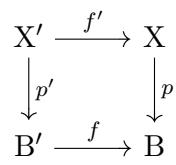
\includegraphics[keepaspectratio]{images/part001_4552bd62.jpg}}

of commutative squares; consider the square

\begin{enumerate}
\def\labelenumi{(\arabic{enumi})}
\setcounter{enumi}{13}
\tightlist
\item
\end{enumerate}

\pandocbounded{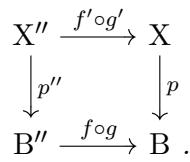
\includegraphics[keepaspectratio]{images/part001_1603e4c4.jpg}}

It is commutative. If squares (12) and (13) are Cartesian, then so is square (14). If squares (13) and (14) are Cartesian, then so is square (12).

Square (14) is commutative, since we have \(p \circ f' \circ g' = f \circ p' \circ g' = f \circ g \circ p''\) . Denote by \(h' : X'' \to B'' \times_{B'} X'\) , \(h : X' \to B' \times_{B} X\) and \(h'' : X'' \to B'' \times_{B} X\) the canonical continuous maps deduced from the commutative squares (12), (13), and (14). Moreover, denote

\[
j \colon \mathrm{B} ^ {\prime \prime} \times_ {\mathrm{B}} \mathrm{X} \rightarrow \mathrm{B} ^ {\prime \prime} \times_ {\mathrm{B} ^ {\prime}} (\mathrm{B} ^ {\prime} \times_ {\mathrm{B}} \mathrm{X})
\]

the continuous map that sends \((b'', x)\) to \((b'', g(b''), x)\) . It is a homeomorphism and one has \(j \circ h'' = (\mathrm{Id}_{\mathrm{B}''} \times_{\mathrm{B}} h) \circ h'\) .

Suppose that square (13) is Cartesian. Then h is a homeomorphism (I, p. 8, prop 2), so the map \(Id_{B''} \times_{B} h\) is a homeomorphism, and \(h''\) is a homeomorphism if and only if \(h'\) is one. This means that square (12) is Cartesian if and only if square (14) is Cartesian (loc. cit.).

With the notation of Proposition 7, one sometimes says that square (14) is the composite square of squares (13) and (12). The first assertion expresses that the composite of two Cartesian squares is Cartesian. In particular, the B''-spaces \(g^{*}(f^{*}(\mathrm{X}))\) and \((f \circ g)^{*}(\mathrm{X})\) are isomorphic.

\pandocbounded{
\includegraphics[keepaspectratio]{images/part001_52f28a70.jpg}}

Remarks. --- 1) It can happen that the squares (12) and (14) are Cartesian without the square (13) being so (I, p. 139, exerc. 2).

\begin{enumerate}
\def\labelenumi{\arabic{enumi})}
\setcounter{enumi}{1}
\tightlist
\item
  Let \(p \colon \mathrm{X} \to \mathrm{B}\) and \(f \colon \mathrm{B}' \to \mathrm{B}\) be continuous maps. The map \(g \colon \mathrm{B}' \to \mathrm{B}' \times \mathrm{B}\) defined by \(g(b') = (b', f(b'))\) is a homeomorphism from \(\mathrm{B}'\) onto the graph \(\mathrm{G}\) of the map \(f\) (TG, I, p. 25, cor. 2), and the fibered product \(\mathrm{B}' \times_{\mathrm{B}} \mathrm{X}\) is identified (I, p. 6) with the subspace of \(\mathrm{B}' \times \mathrm{X}\) that is the inverse image of \(\mathrm{G}\) under the map \(\mathrm{Id}_{\mathrm{B}'} \times p \colon \mathrm{B}' \times \mathrm{X} \to \mathrm{B}' \times \mathrm{B}\) . By the example of I, p. 10 and Corollary 1 of Proposition 5 (I, p. 11), the squares
\end{enumerate}

\[
\begin{array}{c c} \mathrm {B^ {\prime}} \times_ {\mathrm{B}} \mathrm{X} \xrightarrow {i} \mathrm {B^ {\prime}} \times \mathrm{X} & \mathrm {B^ {\prime}} \times \mathrm{X} \xrightarrow {\mathrm{pr} _ {2}} \mathrm{X} \\ \Biggl \downarrow \mathrm{pr} _ {1} & \Biggl \downarrow \mathrm{Id} _ {\mathrm {B^ {\prime}}} \times p \\ \mathrm {B^ {\prime}} \xrightarrow {g} \mathrm {B^ {\prime}} \times \mathrm{B} & \text {et} \end{array} \qquad \qquad \begin{array}{c c} \mathrm {B ^ {\prime}} \times \mathrm{X} \xrightarrow {\mathrm{pr} _ {2}} \mathrm{X} \\ \Biggl \downarrow \mathrm{Id} _ {\mathrm {B^ {\prime}}} \times p & \Biggl \downarrow p \\ \mathrm {B^ {\prime}} \times \mathrm{B} \xrightarrow {\mathrm{pr} _ {2}} \mathrm{B} & \end{array}
\]

(where i denotes the canonical injection) are Cartesian, and the Cartesian square

\[
\begin{array}{c} \mathrm{B} ^ {\prime} \times_ {\mathrm{B}} \mathrm{X} \xrightarrow {\mathrm{pr} _ {2}} \mathrm{X} \\ \Big \downarrow \mathrm{pr} _ {1} \\ \mathrm{B} ^ {\prime} \xrightarrow {f} \mathrm{B} \end{array}
\]

is their composite. In other words, every Cartesian square is identified with the composite square of a Cartesian square obtained by taking a product (I, p. 11, Corollary 1 of Proposition 5, square (8)) and a Cartesian square obtained by passing to subspaces (I, p. 10, example, square (5)).

\begin{enumerate}
\def\labelenumi{\arabic{enumi})}
\setcounter{enumi}{2}
\tightlist
\item
  Let
\end{enumerate}

\[
\begin{array}{c} \mathrm{X} _ {1} \xrightarrow {g _ {1}} \mathrm{X} \\ \Biggl \downarrow p _ {1} \\ \mathrm{B} _ {1} \xrightarrow {f _ {1}} \mathrm{B} \end{array}\tag{15}
\]

and

\[
\begin{array}{c} \mathrm{X} _ {2} \xrightarrow {g _ {2}} \mathrm{X} \\ \Biggl \downarrow p _ {2} \\ \mathrm{B} _ {2} \xrightarrow {f _ {2}} \mathrm{B} \end{array}\tag{16}
\]

  Let

\[
\begin{array}{c} \mathrm{X} _ {1} \times_ {\mathrm{X}} \mathrm{X} _ {2} \xrightarrow {g} \mathrm{X} \\ \Big \downarrow^ {p ^ {\prime}} \\ \mathrm{B} _ {1} \times_ {\mathrm{B}} \mathrm{B} _ {2} \xrightarrow {f} \mathrm{B} \end{array}\tag{17}
\]

where \(f\) (resp. \(g\) ) is the map that defines the structure of a B-space (resp. of an X-space) on the fibered product \(\mathrm{B}_{1} \times_{\mathrm{B}} \mathrm{B}_{2}\) (resp. on the fibered product \(\mathrm{X}_{1} \times_{\mathrm{X}} \mathrm{X}_{2}\) ) and where \(p'\) is the map induced by \(p_{1} \times p_{2}\) by passing to subspaces. It is Cartesian (I, p. 13, Corollary 2 of Proposition 5).

Now consider the following two commutative squares:

\[
\begin{array}{c c} \mathrm{X} _ {1} \times_ {\mathrm{X}} \mathrm{X} _ {2} \xrightarrow {\operatorname{pr} _ {1}} \mathrm{X} _ {1} & \mathrm{X} _ {1} \times_ {\mathrm{X}} \mathrm{X} _ {2} \xrightarrow {\operatorname{pr} _ {2}} \mathrm{X} _ {2} \\ \Biggl \downarrow p ^ {\prime} & \text {and} \\ \mathrm{B} _ {1} \times_ {\mathrm{B}} \mathrm{B} _ {2} \xrightarrow {\operatorname{pr} _ {1}} \mathrm{B} _ {1} & \mathrm{(19)} \\ & \mathrm{B} _ {1} \times_ {\mathrm{B}} \mathrm{B} _ {2} \xrightarrow {\operatorname{pr} _ {2}} \mathrm{B} _ {2}. \end{array}\tag{18}
\]

Square (17) is composed of squares (15) and (18), as well as squares (16) and (19). By prop. 7, squares (18) and (19) are Cartesian.

